\documentclass[]{article}
\usepackage{lmodern}
\usepackage{amssymb,amsmath}
\usepackage{ifxetex,ifluatex}
\usepackage{fixltx2e} % provides \textsubscript
\ifnum 0\ifxetex 1\fi\ifluatex 1\fi=0 % if pdftex
  \usepackage[T1]{fontenc}
  \usepackage[utf8]{inputenc}
\else % if luatex or xelatex
  \ifxetex
    \usepackage{mathspec}
  \else
    \usepackage{fontspec}
  \fi
  \defaultfontfeatures{Ligatures=TeX,Scale=MatchLowercase}
\fi
% use upquote if available, for straight quotes in verbatim environments
\IfFileExists{upquote.sty}{\usepackage{upquote}}{}
% use microtype if available
\IfFileExists{microtype.sty}{%
\usepackage{microtype}
\UseMicrotypeSet[protrusion]{basicmath} % disable protrusion for tt fonts
}{}
\usepackage[margin=1in]{geometry}
\usepackage{hyperref}
\hypersetup{unicode=true,
            pdftitle={Structure to function Regressions},
            pdfauthor={Matthew Flamini},
            pdfborder={0 0 0},
            breaklinks=true}
\urlstyle{same}  % don't use monospace font for urls
\usepackage{color}
\usepackage{fancyvrb}
\newcommand{\VerbBar}{|}
\newcommand{\VERB}{\Verb[commandchars=\\\{\}]}
\DefineVerbatimEnvironment{Highlighting}{Verbatim}{commandchars=\\\{\}}
% Add ',fontsize=\small' for more characters per line
\usepackage{framed}
\definecolor{shadecolor}{RGB}{248,248,248}
\newenvironment{Shaded}{\begin{snugshade}}{\end{snugshade}}
\newcommand{\AlertTok}[1]{\textcolor[rgb]{0.94,0.16,0.16}{#1}}
\newcommand{\AnnotationTok}[1]{\textcolor[rgb]{0.56,0.35,0.01}{\textbf{\textit{#1}}}}
\newcommand{\AttributeTok}[1]{\textcolor[rgb]{0.77,0.63,0.00}{#1}}
\newcommand{\BaseNTok}[1]{\textcolor[rgb]{0.00,0.00,0.81}{#1}}
\newcommand{\BuiltInTok}[1]{#1}
\newcommand{\CharTok}[1]{\textcolor[rgb]{0.31,0.60,0.02}{#1}}
\newcommand{\CommentTok}[1]{\textcolor[rgb]{0.56,0.35,0.01}{\textit{#1}}}
\newcommand{\CommentVarTok}[1]{\textcolor[rgb]{0.56,0.35,0.01}{\textbf{\textit{#1}}}}
\newcommand{\ConstantTok}[1]{\textcolor[rgb]{0.00,0.00,0.00}{#1}}
\newcommand{\ControlFlowTok}[1]{\textcolor[rgb]{0.13,0.29,0.53}{\textbf{#1}}}
\newcommand{\DataTypeTok}[1]{\textcolor[rgb]{0.13,0.29,0.53}{#1}}
\newcommand{\DecValTok}[1]{\textcolor[rgb]{0.00,0.00,0.81}{#1}}
\newcommand{\DocumentationTok}[1]{\textcolor[rgb]{0.56,0.35,0.01}{\textbf{\textit{#1}}}}
\newcommand{\ErrorTok}[1]{\textcolor[rgb]{0.64,0.00,0.00}{\textbf{#1}}}
\newcommand{\ExtensionTok}[1]{#1}
\newcommand{\FloatTok}[1]{\textcolor[rgb]{0.00,0.00,0.81}{#1}}
\newcommand{\FunctionTok}[1]{\textcolor[rgb]{0.00,0.00,0.00}{#1}}
\newcommand{\ImportTok}[1]{#1}
\newcommand{\InformationTok}[1]{\textcolor[rgb]{0.56,0.35,0.01}{\textbf{\textit{#1}}}}
\newcommand{\KeywordTok}[1]{\textcolor[rgb]{0.13,0.29,0.53}{\textbf{#1}}}
\newcommand{\NormalTok}[1]{#1}
\newcommand{\OperatorTok}[1]{\textcolor[rgb]{0.81,0.36,0.00}{\textbf{#1}}}
\newcommand{\OtherTok}[1]{\textcolor[rgb]{0.56,0.35,0.01}{#1}}
\newcommand{\PreprocessorTok}[1]{\textcolor[rgb]{0.56,0.35,0.01}{\textit{#1}}}
\newcommand{\RegionMarkerTok}[1]{#1}
\newcommand{\SpecialCharTok}[1]{\textcolor[rgb]{0.00,0.00,0.00}{#1}}
\newcommand{\SpecialStringTok}[1]{\textcolor[rgb]{0.31,0.60,0.02}{#1}}
\newcommand{\StringTok}[1]{\textcolor[rgb]{0.31,0.60,0.02}{#1}}
\newcommand{\VariableTok}[1]{\textcolor[rgb]{0.00,0.00,0.00}{#1}}
\newcommand{\VerbatimStringTok}[1]{\textcolor[rgb]{0.31,0.60,0.02}{#1}}
\newcommand{\WarningTok}[1]{\textcolor[rgb]{0.56,0.35,0.01}{\textbf{\textit{#1}}}}
\usepackage{graphicx,grffile}
\makeatletter
\def\maxwidth{\ifdim\Gin@nat@width>\linewidth\linewidth\else\Gin@nat@width\fi}
\def\maxheight{\ifdim\Gin@nat@height>\textheight\textheight\else\Gin@nat@height\fi}
\makeatother
% Scale images if necessary, so that they will not overflow the page
% margins by default, and it is still possible to overwrite the defaults
% using explicit options in \includegraphics[width, height, ...]{}
\setkeys{Gin}{width=\maxwidth,height=\maxheight,keepaspectratio}
\IfFileExists{parskip.sty}{%
\usepackage{parskip}
}{% else
\setlength{\parindent}{0pt}
\setlength{\parskip}{6pt plus 2pt minus 1pt}
}
\setlength{\emergencystretch}{3em}  % prevent overfull lines
\providecommand{\tightlist}{%
  \setlength{\itemsep}{0pt}\setlength{\parskip}{0pt}}
\setcounter{secnumdepth}{0}
% Redefines (sub)paragraphs to behave more like sections
\ifx\paragraph\undefined\else
\let\oldparagraph\paragraph
\renewcommand{\paragraph}[1]{\oldparagraph{#1}\mbox{}}
\fi
\ifx\subparagraph\undefined\else
\let\oldsubparagraph\subparagraph
\renewcommand{\subparagraph}[1]{\oldsubparagraph{#1}\mbox{}}
\fi

%%% Use protect on footnotes to avoid problems with footnotes in titles
\let\rmarkdownfootnote\footnote%
\def\footnote{\protect\rmarkdownfootnote}

%%% Change title format to be more compact
\usepackage{titling}

% Create subtitle command for use in maketitle
\providecommand{\subtitle}[1]{
  \posttitle{
    \begin{center}\large#1\end{center}
    }
}

\setlength{\droptitle}{-2em}

  \title{Structure to function Regressions}
    \pretitle{\vspace{\droptitle}\centering\huge}
  \posttitle{\par}
    \author{Matthew Flamini}
    \preauthor{\centering\large\emph}
  \postauthor{\par}
      \predate{\centering\large\emph}
  \postdate{\par}
    \date{March 21, 2019}


\begin{document}
\maketitle

\hypertarget{anneal-regression}{%
\subsection{Anneal Regression}\label{anneal-regression}}

I was able to get a very good fit using am multiple regression model.
High correlation, low p value, and very good ``goodness of fit'' stats,
indicating that the data was not over fit.

\begin{Shaded}
\begin{Highlighting}[]
\NormalTok{anneal.UTS <-}\StringTok{ }\KeywordTok{lm}\NormalTok{(UTS_FTIR }\OperatorTok{~}\StringTok{ }\NormalTok{wamor_or }\OperatorTok{+}\StringTok{ }\NormalTok{wcryst_or }\OperatorTok{+}\StringTok{ }\NormalTok{tot_or, }\DataTypeTok{data =}\NormalTok{ min.anneal)}
\KeywordTok{summary}\NormalTok{(multiUTS)}
\end{Highlighting}
\end{Shaded}

\begin{verbatim}
## 
## Call:
## lm(formula = UTS_FTIR ~ poly(Perc_Cryst, 3, raw = TRUE), data = min.quench)
## 
## Residuals:
##       633       956      1279      1565      1973      2435      2632 
## -0.110073 -0.008719  0.012468  0.100013 -0.003493  0.002235 -0.002216 
##      2791 
##  0.009783 
## 
## Coefficients:
##                                    Estimate Std. Error t value Pr(>|t|)  
## (Intercept)                      -1.671e+02  5.580e+01  -2.994   0.0402 *
## poly(Perc_Cryst, 3, raw = TRUE)1  8.492e+00  2.756e+00   3.082   0.0369 *
## poly(Perc_Cryst, 3, raw = TRUE)2 -1.428e-01  4.513e-02  -3.165   0.0340 *
## poly(Perc_Cryst, 3, raw = TRUE)3  7.974e-04  2.452e-04   3.252   0.0313 *
## ---
## Signif. codes:  0 '***' 0.001 '**' 0.01 '*' 0.05 '.' 0.1 ' ' 1
## 
## Residual standard error: 0.07495 on 4 degrees of freedom
## Multiple R-squared:  0.9204, Adjusted R-squared:  0.8607 
## F-statistic: 15.42 on 3 and 4 DF,  p-value: 0.01155
\end{verbatim}

\begin{Shaded}
\begin{Highlighting}[]
\KeywordTok{model_fit_stats}\NormalTok{(multiUTS)}
\end{Highlighting}
\end{Shaded}

\begin{verbatim}
##   r.squared adj.r.squared pred.r.squared      press      AIC      BIC
## 1  0.920423     0.8607402      0.8304482 0.04787185 -14.2978 -13.9006
\end{verbatim}

\hypertarget{quench-regression}{%
\subsection{Quench Regression}\label{quench-regression}}

I could not get the same model to work with the quench data. However, I
got a different model that works quite well, and is also suggested by
the data. Here I use a 3rd degree polynomial, but it looks like once we
increase our sample size, a second degree will fit nicely. Like before,
the model has a high predictive value, and does not seem to be over fit
based on both the eye test and the fit stats

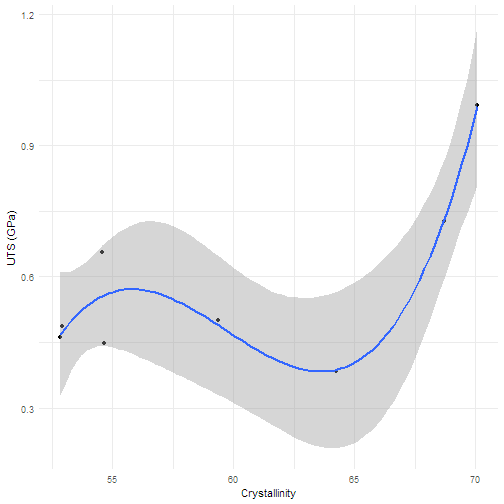
\includegraphics{knitTest_files/figure-latex/Quench Plot-1.pdf}

\begin{Shaded}
\begin{Highlighting}[]
\NormalTok{multiUTS <-}\StringTok{ }\KeywordTok{lm}\NormalTok{(UTS_FTIR }\OperatorTok{~}\StringTok{ }\KeywordTok{poly}\NormalTok{(Perc_Cryst , }\DecValTok{3}\NormalTok{, }\DataTypeTok{raw =} \OtherTok{TRUE}\NormalTok{), }\DataTypeTok{data =}\NormalTok{ min.quench)}
\KeywordTok{summary}\NormalTok{(multiUTS)}
\end{Highlighting}
\end{Shaded}

\begin{verbatim}
## 
## Call:
## lm(formula = UTS_FTIR ~ poly(Perc_Cryst, 3, raw = TRUE), data = min.quench)
## 
## Residuals:
##       633       956      1279      1565      1973      2435      2632 
## -0.110073 -0.008719  0.012468  0.100013 -0.003493  0.002235 -0.002216 
##      2791 
##  0.009783 
## 
## Coefficients:
##                                    Estimate Std. Error t value Pr(>|t|)  
## (Intercept)                      -1.671e+02  5.580e+01  -2.994   0.0402 *
## poly(Perc_Cryst, 3, raw = TRUE)1  8.492e+00  2.756e+00   3.082   0.0369 *
## poly(Perc_Cryst, 3, raw = TRUE)2 -1.428e-01  4.513e-02  -3.165   0.0340 *
## poly(Perc_Cryst, 3, raw = TRUE)3  7.974e-04  2.452e-04   3.252   0.0313 *
## ---
## Signif. codes:  0 '***' 0.001 '**' 0.01 '*' 0.05 '.' 0.1 ' ' 1
## 
## Residual standard error: 0.07495 on 4 degrees of freedom
## Multiple R-squared:  0.9204, Adjusted R-squared:  0.8607 
## F-statistic: 15.42 on 3 and 4 DF,  p-value: 0.01155
\end{verbatim}

\begin{Shaded}
\begin{Highlighting}[]
\KeywordTok{model_fit_stats}\NormalTok{(multiUTS)}
\end{Highlighting}
\end{Shaded}

\begin{verbatim}
##   r.squared adj.r.squared pred.r.squared      press      AIC      BIC
## 1  0.920423     0.8607402      0.8304482 0.04787185 -14.2978 -13.9006
\end{verbatim}

\hypertarget{pca-of-anneal-and-quench}{%
\subsection{PCA of Anneal and Quench}\label{pca-of-anneal-and-quench}}

In order to determine whether the Quench and Anneal samples differ in
some way, I decided to perform PCA on them to determine if they are
really distinct populations of fibers. That is to say, an annealed fiber
is different than a quenched fiber.

\begin{Shaded}
\begin{Highlighting}[]
\NormalTok{pca.all.df  <-}\StringTok{ }\KeywordTok{prcomp}\NormalTok{(pca.all, }\DataTypeTok{scale =} \OtherTok{TRUE}\NormalTok{, }\DataTypeTok{center =} \OtherTok{TRUE}\NormalTok{)}
\end{Highlighting}
\end{Shaded}

\begin{verbatim}
## pdf 
##   2
\end{verbatim}

\includegraphics{C:/Users/Matt/Google Drive/Education/Rowan/BME/Research/autofibers/quenchVsAnnealPCA.png}

\hypertarget{stress-strain-curves}{%
\subsection{Stress Strain Curves}\label{stress-strain-curves}}

In order to visualize the changes in strength as a function of
temperatire, I have arranged the stress strain curves and thier
derivitivesside by side according to the temperature they were treated.

\hypertarget{anneal}{%
\subsubsection{Anneal}\label{anneal}}

\begin{verbatim}
## TableGrob (2 x 1) "arrange": 2 grobs
##   z     cells    name           grob
## 1 1 (1-1,1-1) arrange gtable[layout]
## 2 2 (2-2,1-1) arrange gtable[layout]
\end{verbatim}

\begin{verbatim}
## pdf 
##   2
\end{verbatim}

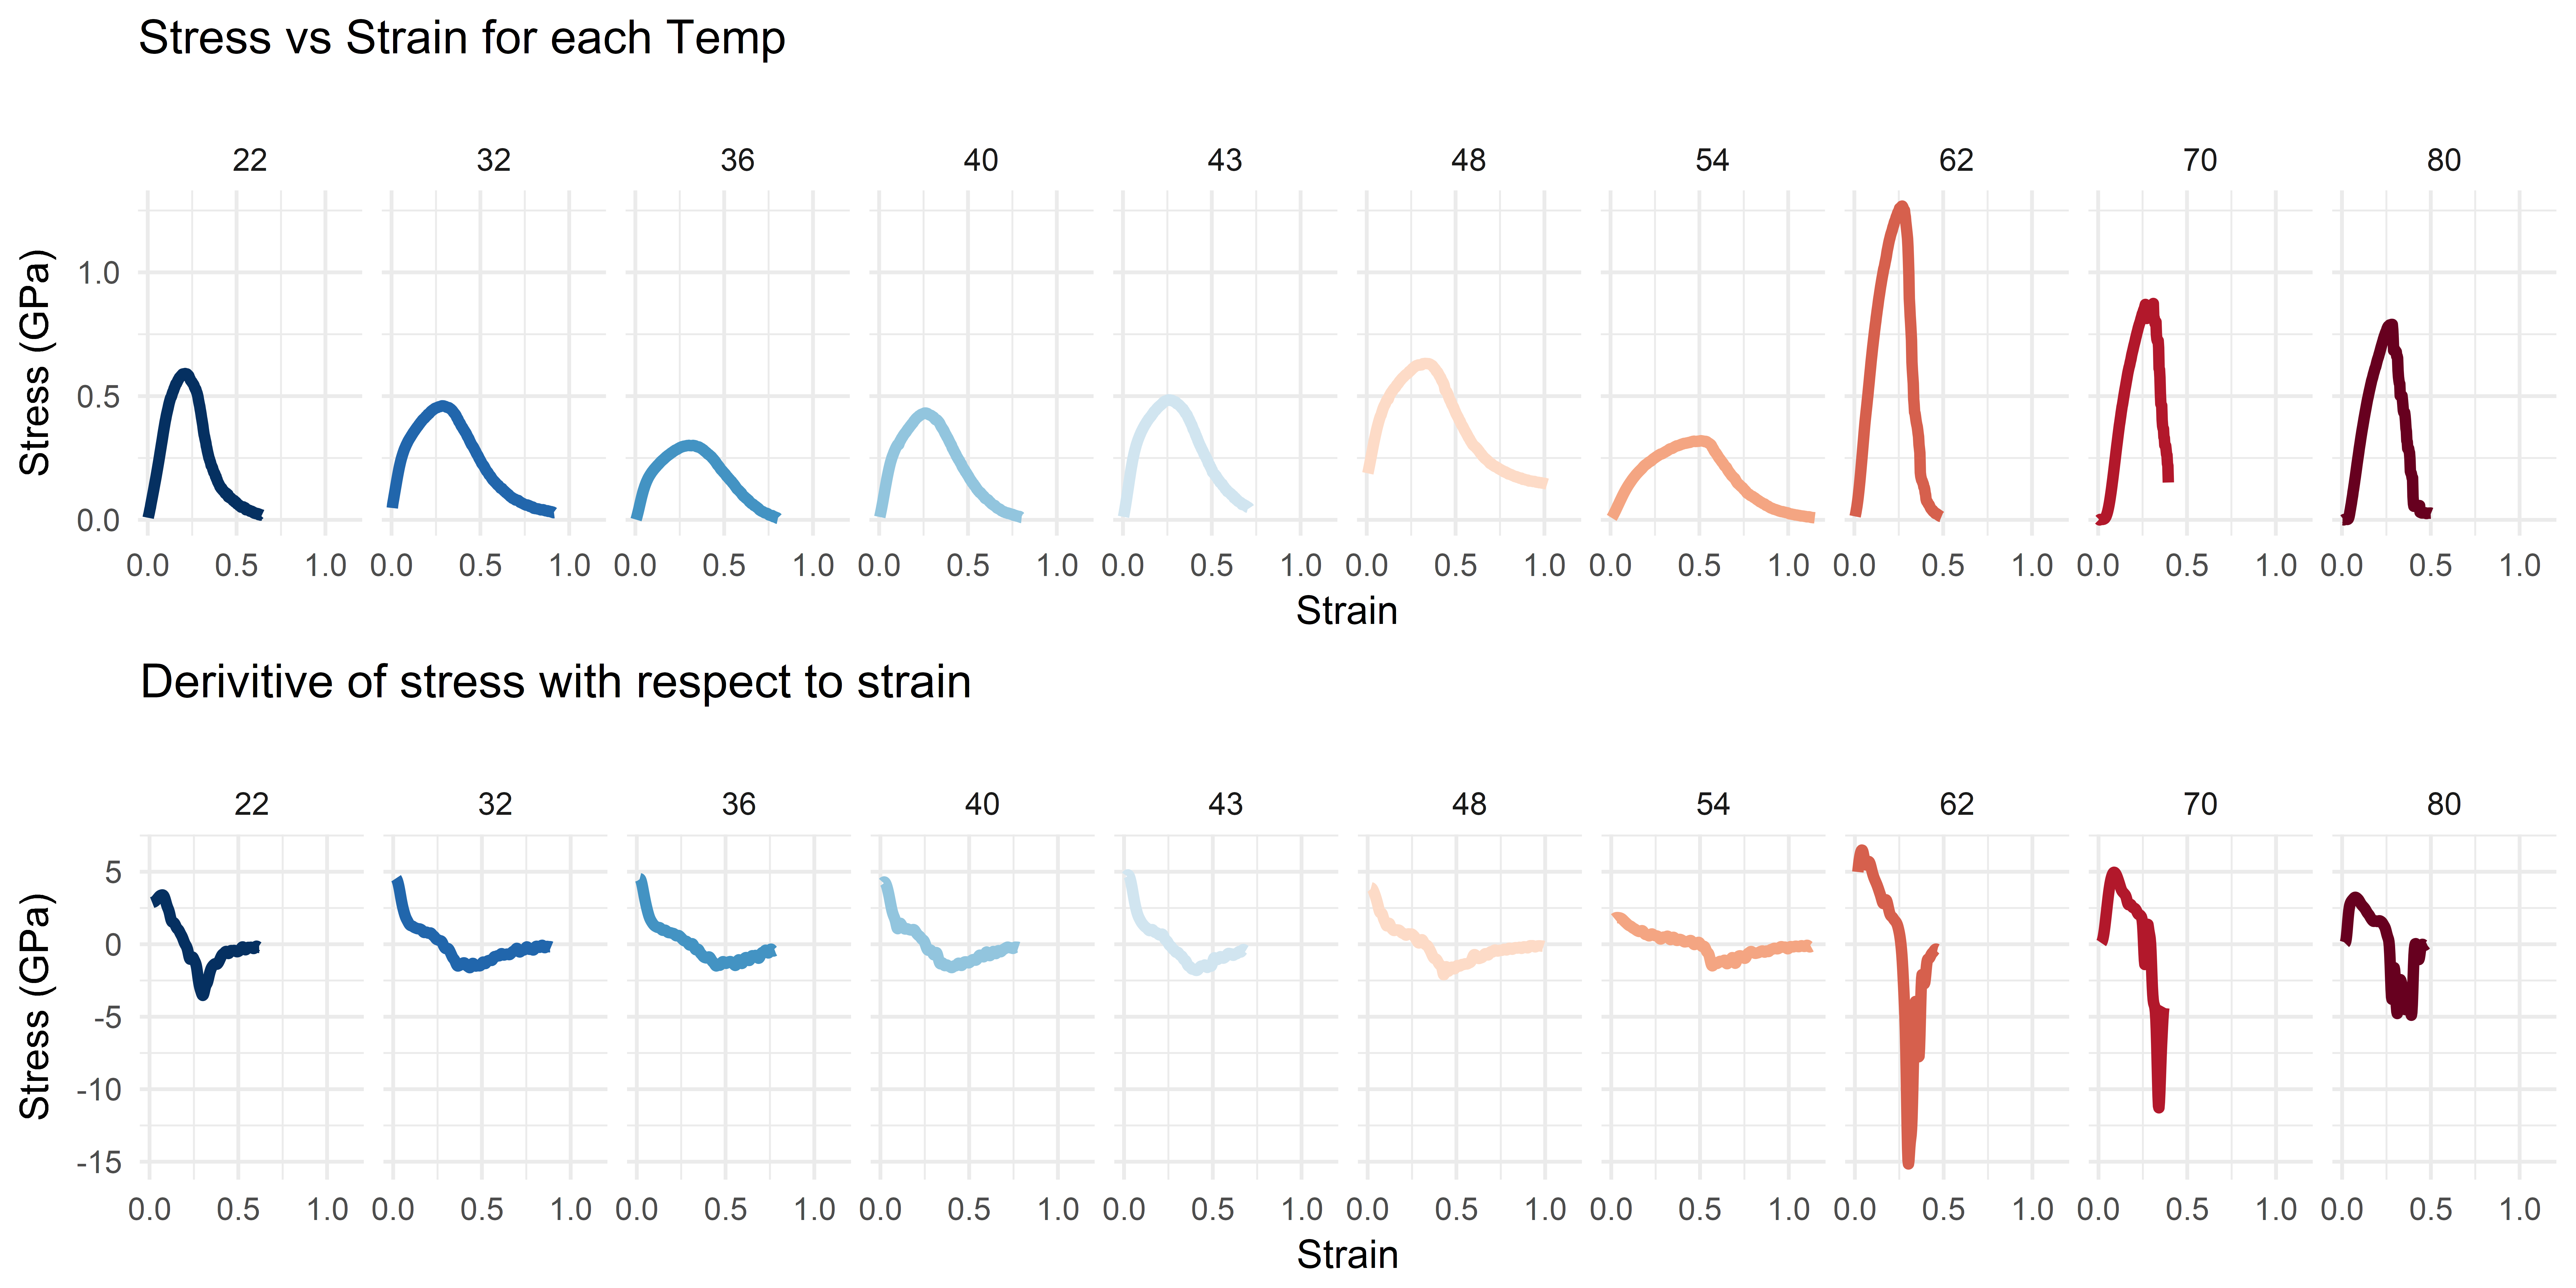
\includegraphics{C:/Users/Matt/Google Drive/Education/Rowan/BME/Research/autofibers/ymAndssSequentialanneal.png}

\hypertarget{quench}{%
\subsubsection{Quench}\label{quench}}

\begin{verbatim}
## pdf 
##   2
\end{verbatim}

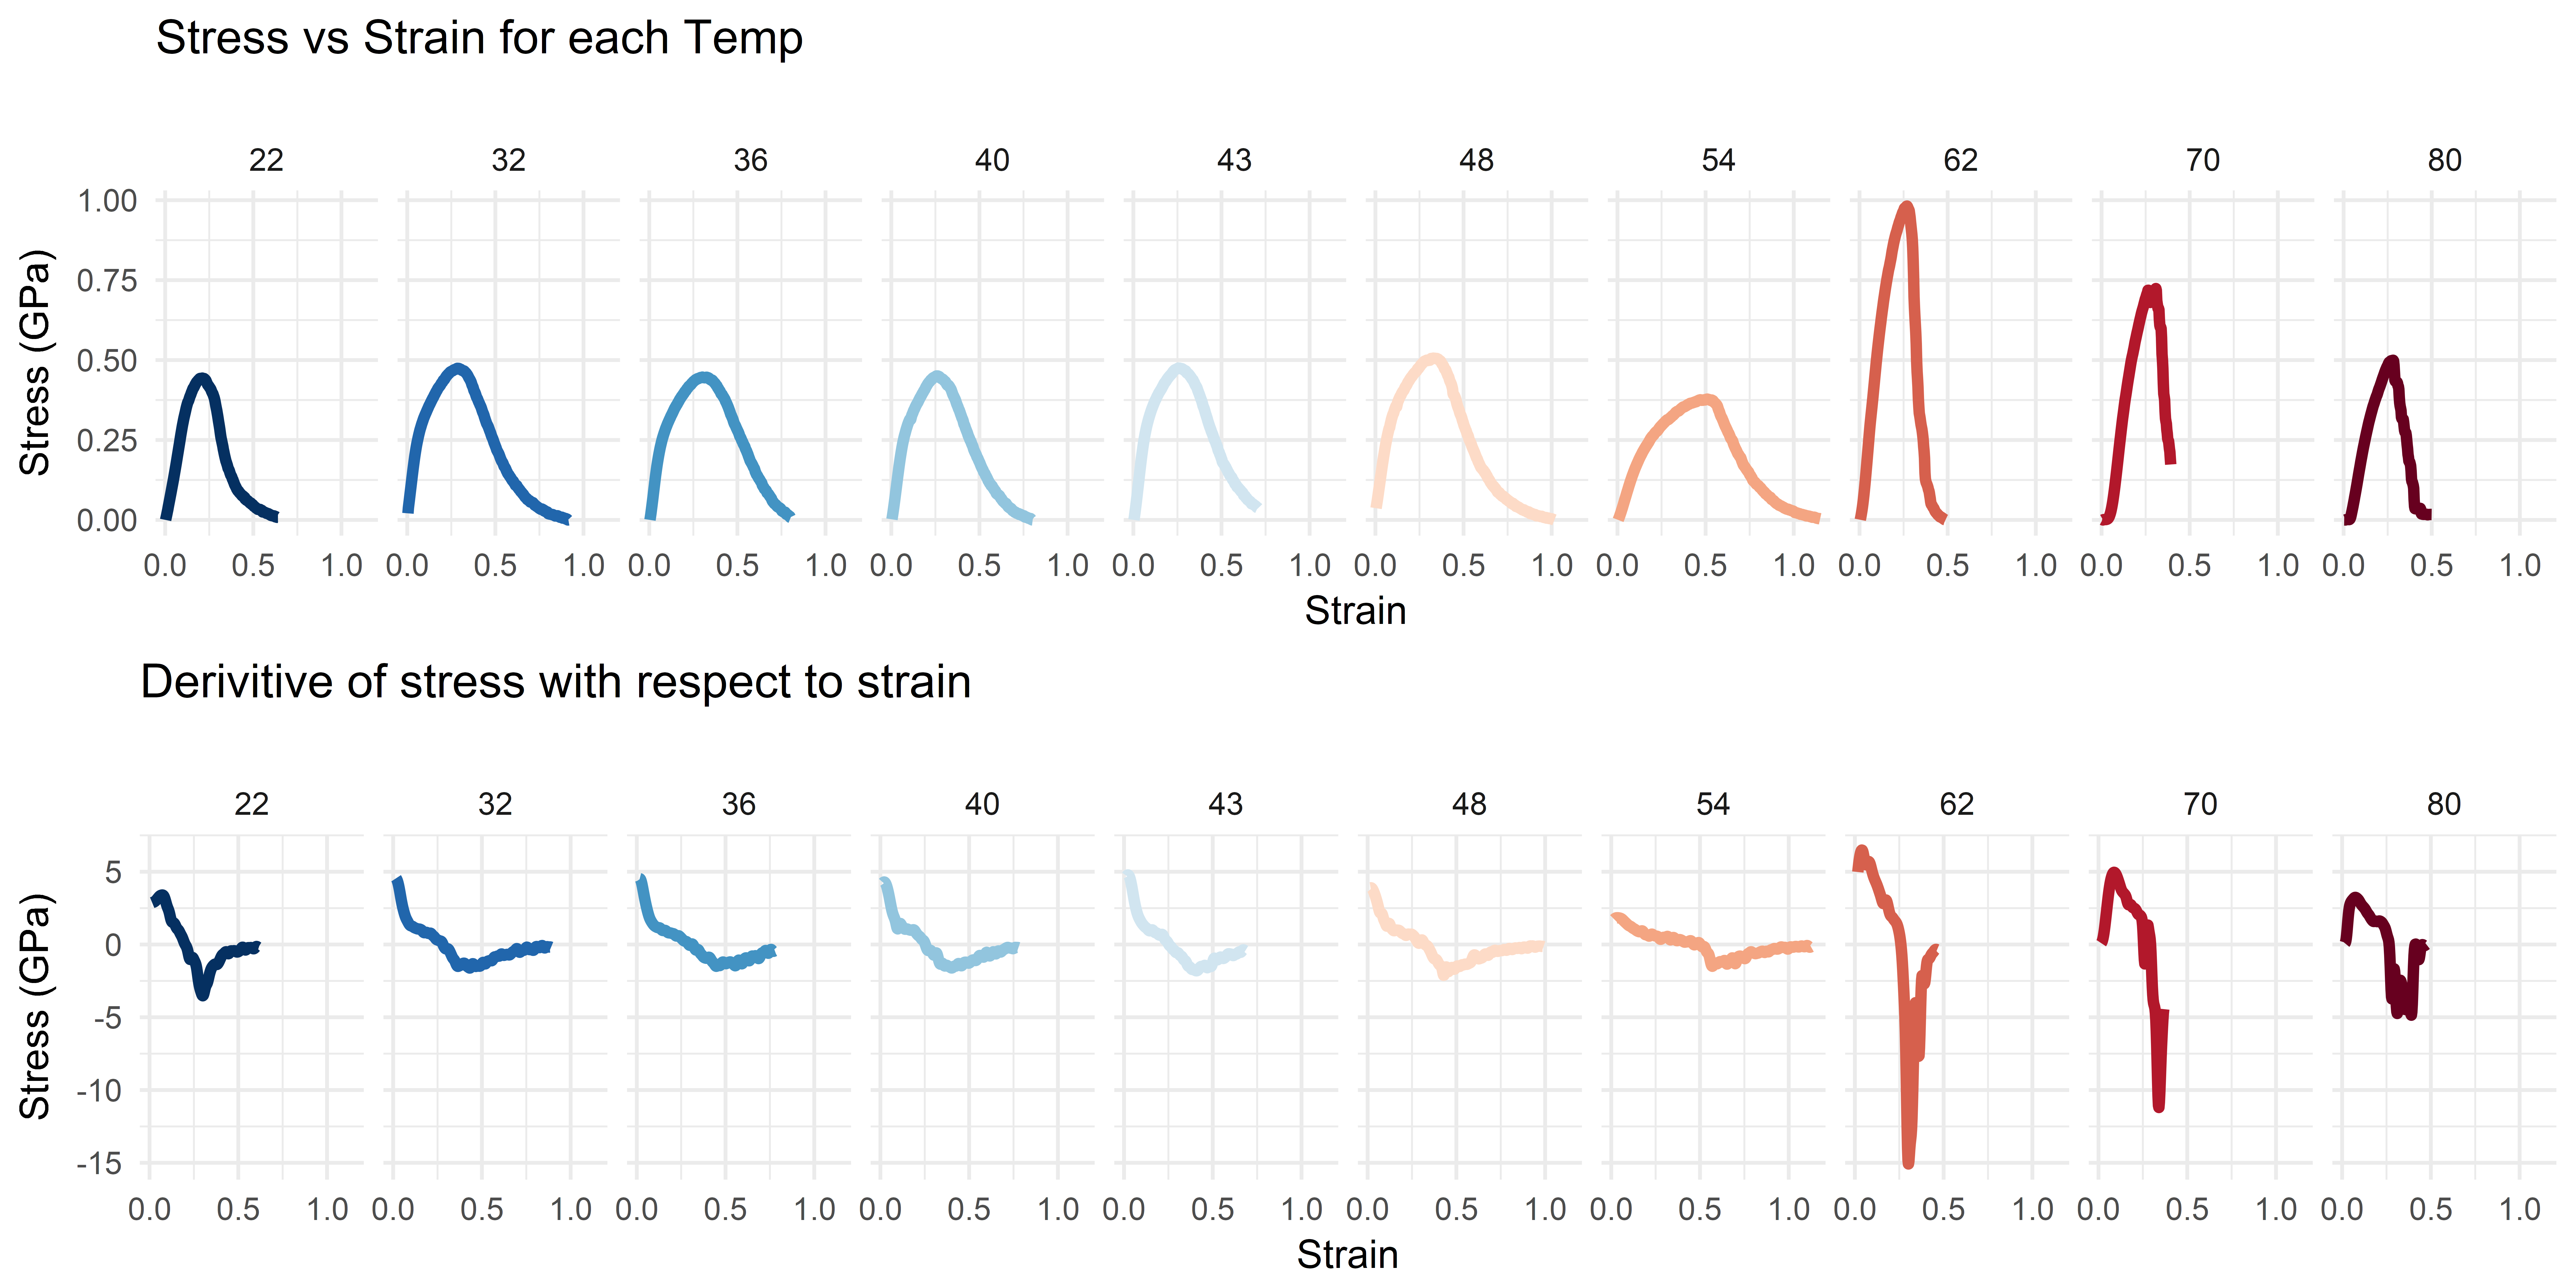
\includegraphics{C:/Users/Matt/Google Drive/Education/Rowan/BME/Research/autofibers/ymAndssSequentialquench.png}


\end{document}
